%=====================================================================================================

%       Math 244 Lecture Notes

%       Chapter 20

%				201701

%				LaTeX=>PDF sizing, graphics
%=====================================================================================================


\documentclass[12pt]{amsart}
\usepackage{amssymb,latexsym}
\usepackage{graphicx}
\usepackage{multicol}
\usepackage{multirow}
\usepackage{amsmath}
\usepackage{calc}
\usepackage{enumitem}
\usepackage{fancyhdr,lastpage}
\usepackage{setspace}
\usepackage{caption}
\usepackage{framed}
\usepackage{wasysym}

\theoremstyle{definition}
\pagestyle{fancy}
\newtheorem{theorem}{Theorem}
\newtheorem{lemma}{Lemma}
\newtheorem{defi}{Definition}
\newtheorem*{notation}{Notation}
\newtheorem{ex}{Example}
\newtheorem{proc}{Process}
\newtheorem{gw}{Group Work}
\newtheorem*{summary}{}

\setlength{\textwidth}{7.25in}			%for =>PDF, use 6.5in
\setlength{\textheight}{9.5in}		%for =>PDF, use 9.5in
\setlength{\oddsidemargin}{-0.375in}		
\setlength{\evensidemargin}{-0.375in}		
\setlength{\voffset}{-.75in}			%for=>PDF, use -0.75in
\setlength{\footskip}{15pt}


% For degree symbol
\newcommand{\degree}{\ensuremath{^\circ}}



% enumerate settings
\setlist{itemsep=4pt}	%topsep=0.1em
\renewcommand{\labelenumi}{ (\alph{enumi}) }			% makes enumeration (a) instead of (a).



\usepackage{placeins} % enables \FloatBarrier, useful for positioning figures/tables more precisely.
%\usepackage[dvips]{graphics}
%\usetikzlibrary{arrows}


\usepackage{pst-func}


\usepackage{hyperref}
%\usepackage{url}
\hypersetup{colorlinks=true,urlcolor=blue,linkcolor=blue,breaklinks=true}

\usepackage{xcolor}
%		My colors
\definecolor{silver}{rgb}{0.95,0.95,0.95}
\definecolor{mypurple}{cmyk}{0.5,1,0,0}			%purple
\definecolor{myblue}{cmyk}{1,0.012,0,0}		%blue
\definecolor{mygreen}{cmyk}{1,0,0.99995,0}		%green
\definecolor{myred}{cmyk}{0,1,1,0}


\setlength{\parindent}{0pt}

\date{}



\begin{document}

\newcommand{\ph}{\phantom}
\newcommand{\ds}{\displaystyle}

\renewcommand{\emph}{\textbf}
\onehalfspace

%============================================================
%           Header Stuff   CHANGE FOR EACH SECTION!!!
%============================================================

\fancyhf{}   % clears both header and footer
\fancyfoot[RE,RO]{ \scriptsize{Page \thepage\ of \pageref{LastPage}}}
\fancyfoot[LE,LO]{\scriptsize{Instructor:  J.Wherry}}
\fancyhead[RE,RO]{\scriptsize{Chapter 20: Confidence Intervals for One Average }}
\fancyhead[LE,LO]{\scriptsize{Math 244 Lecture Notes }}
\renewcommand{\headrulewidth}{0.4pt} % Removes header line if 0pt
\fancyfootoffset[LE,LO]{0in}        %Moves center ??
\renewcommand{\footrulewidth}{0.4pt} % Removes header line if 0pt



%============================================================
%           Title/ Info
%============================================================

\begin{center}

	\larger[3]	Math 244 Lecture Notes \smaller[3]		\\[22pt]

\end{center}

\section*{Chapter 20: Confidence Intervals for One Average}




 \textbf{Overview:} We just finished looking at singular and multiple proportions. Today, however, we begin doing inference for means/averages.\\
 ~\\
 As a reminder, confidence intervals in general look like (Center)$\pm$(Dist$)^*$SE. So, assuming we have a model that looks at averages, we should be good to go. And, well, we do!
 
 \begin{framed}
 The \emph{Central Limit Theorem} states that $$\bar{X}=N\left(\mu,\frac{\sigma}{\sqrt{n}}\right)$$ assuming that
 \begin{enumerate}
  \item \,
  \item \,
  \item \,
 \end{enumerate}

 \end{framed}

 In short, it tells us that regardless of the original distribution $X$, we should expect the distribution for the sample averages to look normal for large $n$. As $n$ gets larger, the distribution will look more and more normal.\\
 ~\\
 \begin{ex} Using the distribution above and the fact that confidence intervals are based off samples, create the formula for the CI for $\mu$.\end{ex}
 
 \vspace{1in}
 
 WARNING: $\bar{x}\approx \mu$ but $\sigma$ and $s$ are not interchangeable (it's a biased estimator). The two values are only close for VERY large $n$.
 \newpage
 \noindent Okay. We have a confidence interval, but it doesn't work for most values of $n$. What's the fix? A new distribution!
 
 \begin{framed}
 \emph{Student t-Distribution} is like a normal distribution, but it has a built-in error correcter to deal with small sample sizes. Using it, we can rewrite the CLT as $$\bar{X}=t_{df}\left(\mu,\frac{s}{\sqrt{n}}\right)$$
 \end{framed}
 
If you switch $\sigma$ for $s$, then change $Z$ to $t$. That's pretty much it. For example, our CI was $\bar{x}\pm Z^* \frac{\sigma}{\sqrt{n}}$. Now we have the following:
\begin{framed}
 A confidence interval for $\mu$ based off sample information $\bar{x}$ and $s$ can be found using $$\bar{x}\pm t^*_{df} \frac{s}{\sqrt{n}}$$ assuming that
  \begin{enumerate}
  \item \,
  \item \,
  \item \,
 \end{enumerate}
\end{framed}

Problem almost solved. There's just the matter of finding $t^*$.\\
~\\
\textbf{Degrees of Freedom:}
\vspace{2in}

In general, $df=$\\
~\\
\newpage
There is a different $t$-distribution for each $df$. That's like having a different normal type distribution for infinitely many different values of $n$. So, if we want to find the critical values, we need either a table for every possible value for $n$ OR a critical value table that works for most values of $n$.\\
~\\
Using the Critical Value table: Determine the $df$. Determine the $C$-level. Use the $t^*$ value in the table where the $df$ row meets the $C$ column.\\

\begin{ex} Find $t^*$ if $C=90\%$ and $n=16$\end{ex}
\begin{ex} Find $t^*$ if $C=95\%$ and $n=51$\end{ex}
\begin{ex} Find $t^*$ if $C=99\%$ and $n=500$\end{ex}
\begin{ex} Find $t^*$ if $C=92\%$ and $n=30$\end{ex}
\begin{ex} Find $t^*$ if $C=99\%$ and $n=10000$\end{ex}

 OBSERVATION: For large $n$...\underline{\hspace{2in}}\\
 ~\\
 
 Below are pictures of the $t$-distribution for $df=1$ (dashed) and $df=12$ (solid) to give you some context. 
 
 \psset{xunit=1cm,yunit=10cm}
\begin{pspicture*}(-6,-0.1)(6,0.5)
\psaxes[Dy=0.1]{->}(0,0)(-5,0)(5.5,0.5)
\psset{linewidth=1pt,plotpoints=100}
\psTDist[linecolor=blue,nue=12]{-5}{5}
\psTDist[linestyle=dashed,nue=1]{-5}{5}
\end{pspicture*}
\newpage

In general, the $t$-distribution is like a short and stocky version of the normal distribution. Small values of $n$ give larger interval. However, as $n$ increases, the graph will look more and more normal. The graph has several $t$-distributions with increasing $n$ and a solid normal distribution.

\begin{pspicture*}(-6,-0.1)(6,0.5)
\psaxes[Dy=0.1]{->}(0,0)(-5,0)(5.5,0.5)
\psset{linewidth=1pt,plotpoints=100}
\psGauss[linecolor=blue,mu=0,sigma=1]{-5}{5}
\psTDist[linestyle=dashed,nue=1]{-5}{5}
\psTDist[linestyle=dashed,nue=2]{-5}{5}
\psTDist[linestyle=dashed,nue=3]{-5}{5}
\psTDist[linestyle=dashed,nue=100]{-5}{5}
\end{pspicture*}
\\
\hrule
\vspace{0.1in}
Okay, we now have a way to find $t*$ in the formula $\bar{x}\pm t^*_{df} \frac{s}{\sqrt{n}}$. Let's find some confidence intervals!
\begin{ex} If $\bar{x}=18$in, $s=20$in, and $n=31$, create a $90\%$ CI for $\mu$.\end{ex}
\vspace{1.5in}

\begin{ex} Mr. Wherry weighs $100$ cats and find that they have an average weight of $8.5$ pounds with a standard deviation of $1.8$ lbs. Assuming that the sample is representative, create a $95\%$ CI for $\mu$ \end{ex}
\vspace{1.5in}
\newpage

\begin{ex} The average cost of $15$ cars is found to be $\$26,000$ with a SD of $\$500$. Why can we not create a CI with just this information?\end{ex}
\vspace{1.5in}

\begin{ex} How many students does the average PCC Rock Creek student take? Survey time!\end{ex}
\vspace{3in}

\newpage
\noindent \textbf{Checking work with Calculator:} In our calculator, we use ``tInt" to check our interval. This is found in either [Stat]$\rightarrow$[Tests] on the TI-83/84 OR [Stat/List]$\rightarrow$[F7:Ints] on the TI-89. Type in your relevant information and you are good to go!\\
~\\
Calc Interval for PCC student information:

\begin{ex}
	The Oregon Zoo is curious how much on average people spend on food. A worker performs a survey and finds that out of $200$ people sampled (various days and times) that spent $\$10.72$ per person on average with a standard deviation of $\$1.35$. Create a $95\%$ confidence interval for the true average amount that people spend on food.
\end{ex}

\begin{ex}
	The owners of Cinetopia want to know the average length of feature films. They sample $100$ movies from the last $4$ years and find that they have an average run length of $100\,mins$ with a standard deviation of $18\,mins$. Create a $90\%$ confidence interval for the true average film length.
\end{ex}

\begin{ex}
	Barry Allen is training for the mile. In a recent study at STAR Labs, it was determined that he's running an average mile time of $0.1$ second with a standard deviation of $0.01$ seconds for a collection of $52$ samples. Using this information and assuming that his sample is representative, create a $99\%$ confidence interval for his mile time.
\end{ex}

\begin{ex}
	Claire works as a night nurse. She samples $50$ individuals and finds that they have an average hospital bill of $\$3,200$ for one night with a standard deviation of $\$700$. Using this information, create a $90\%$ for the true average cost per night at the hospital.
\end{ex}

\begin{ex}
	Mr. Wherry is training his cat, Fiona, for the Cat Olympics. She is known for her high jump. Curious as to what her true average high jump height is, Mr. Wherry measures several jump heights and gets the following data in feet: $4.5$, $4.75$, $4.75$, $4.8$, $4.8$, $4.8$, $4.8$, $5$, $5$, and $5.25$. Create a $95\%$ for the true average jump height. [Picture included for educational purposes]
\end{ex}

\begin{figure}[h]
 \centering
 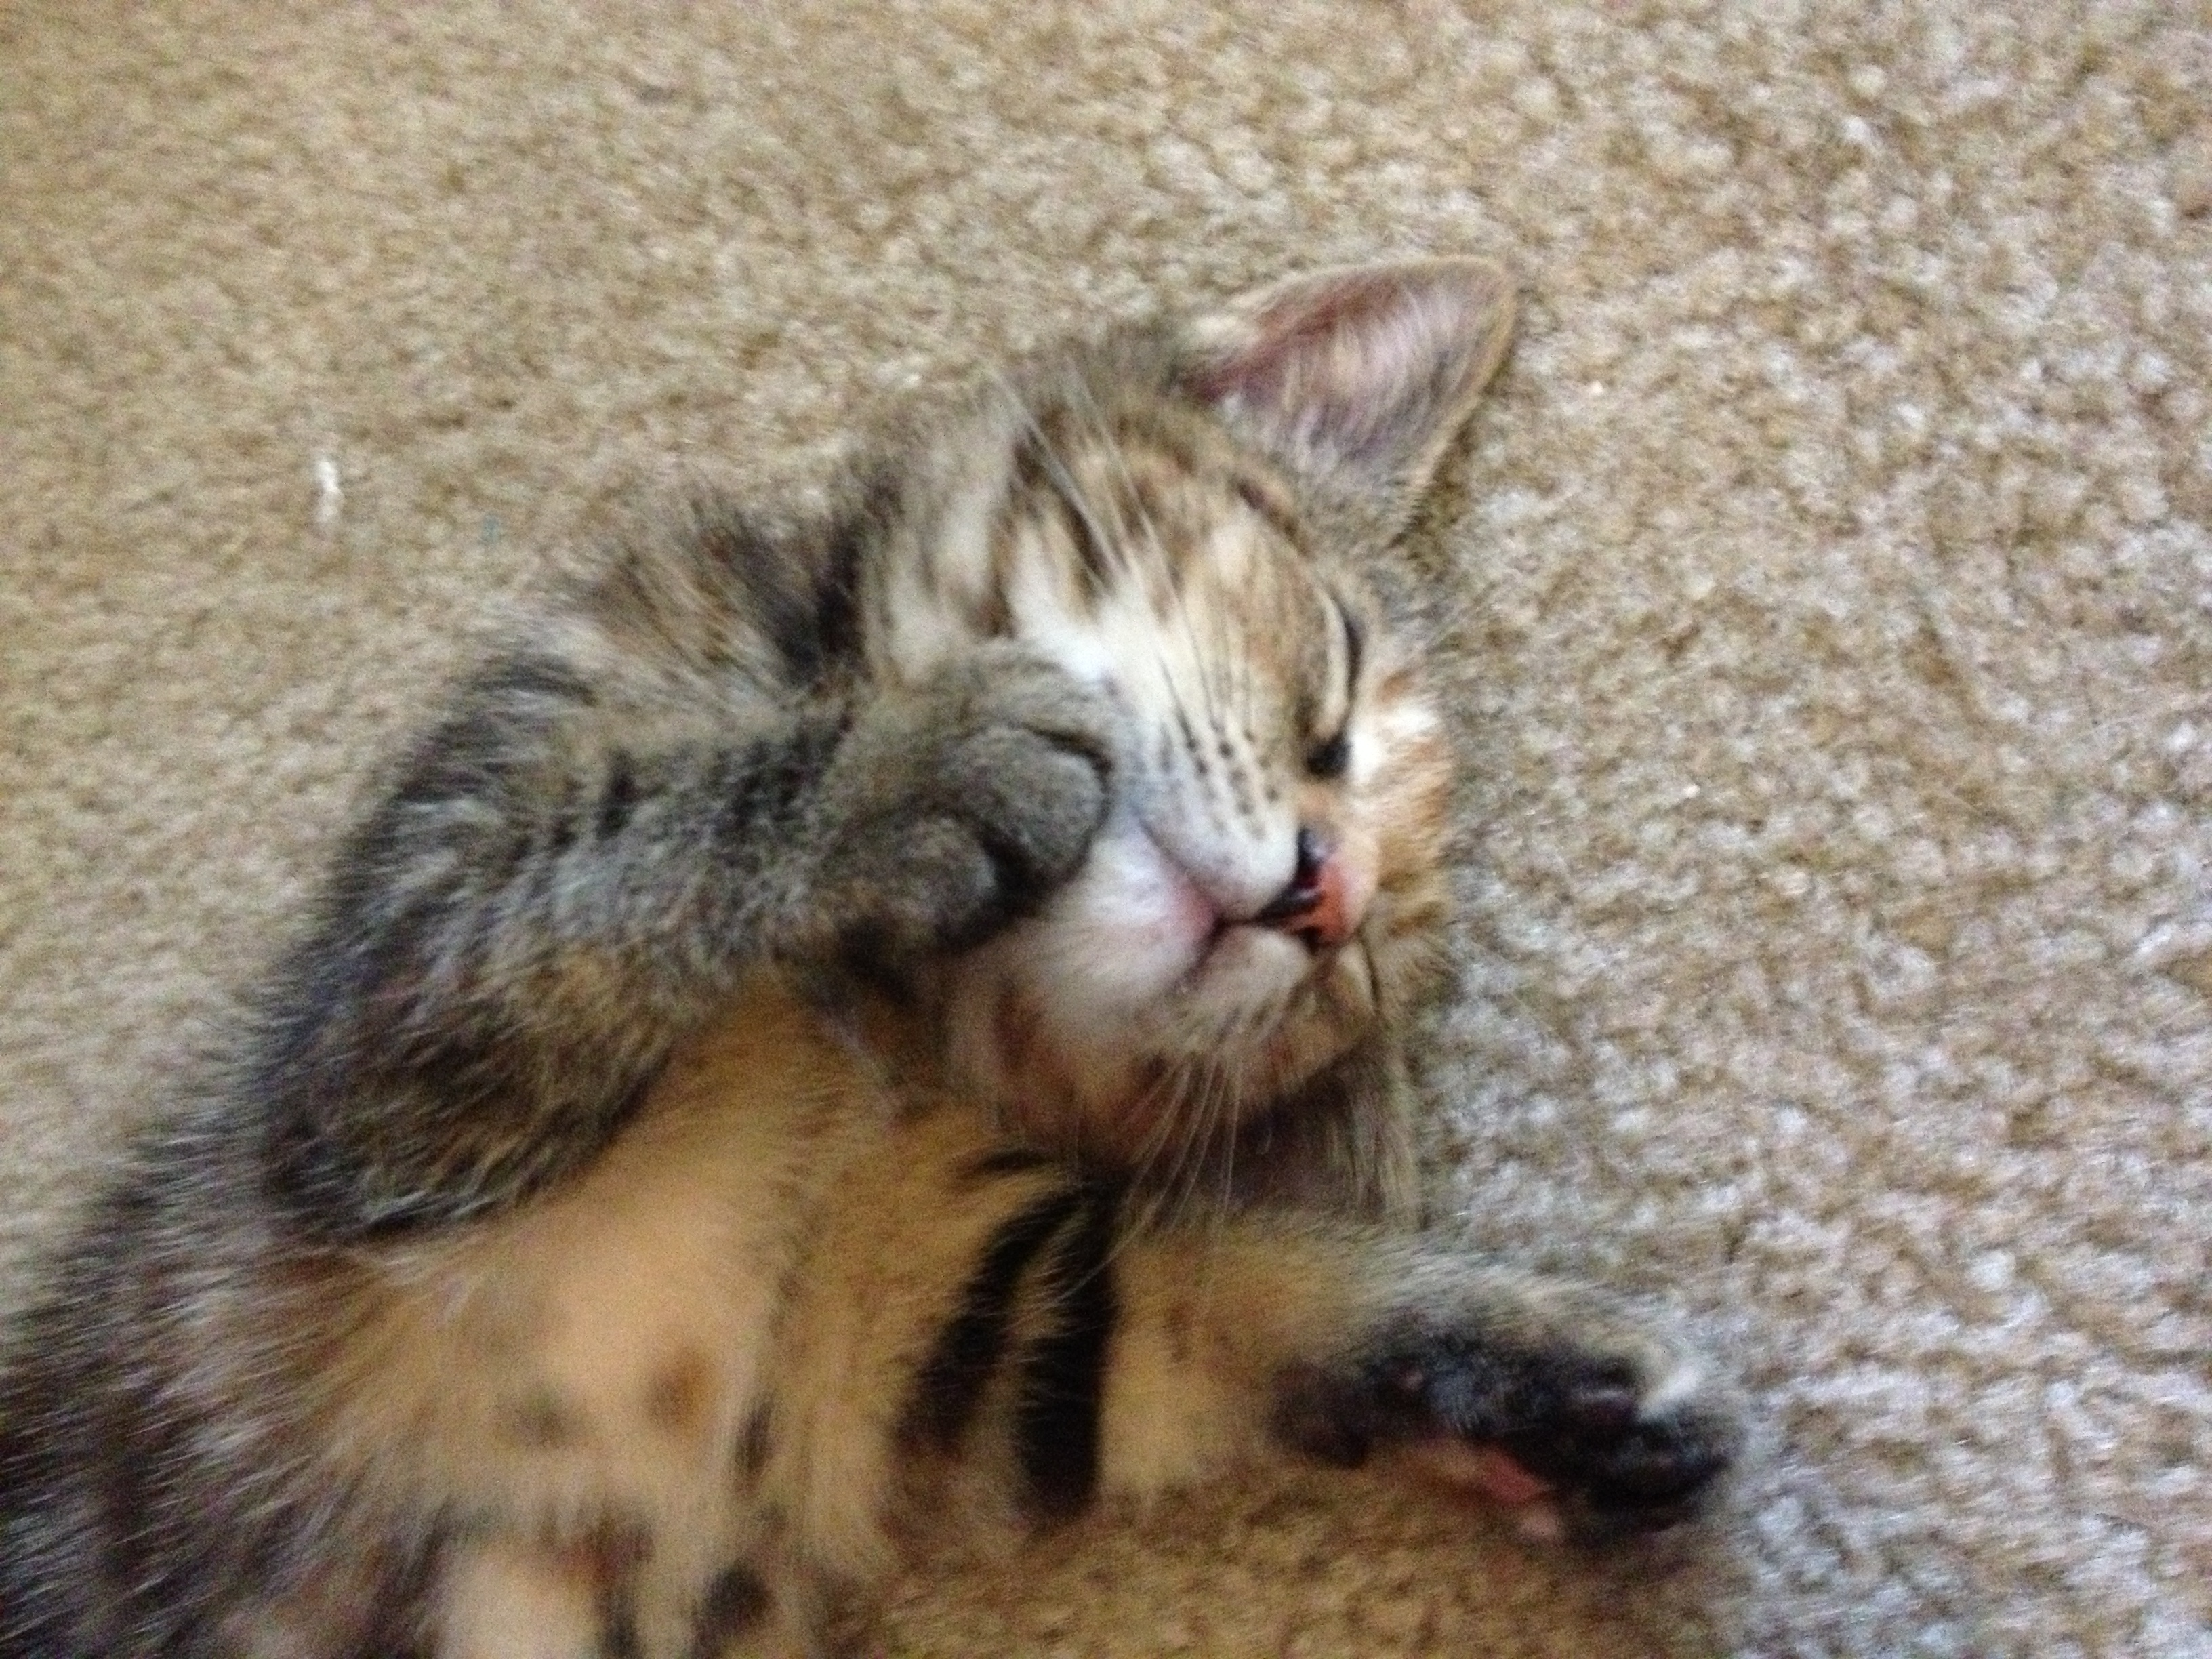
\includegraphics[width=2.5in,keepaspectratio=true]{./IMG_0929.JPG}
 % IMG_0929.JPG: 0x0 pixel, 0dpi, 0.00x0.00 cm, bb=
 \label{fig: Fiona}
\end{figure}

\end{document}
